\chapter{Dialogbeispiel}
\label{chapter-dialogbeispiel}

Der folgende Abschnitt präsentiert das in der vorliegenden Arbeit realisierte System anhand eines
beispielhaften Nutzungsszenarios. Das Szenario Start mit Mila, einer Erstsemester Studentin im
Studiengang Medieninformatik. Mila belegt im ersten Semester das Modul \textit{\ac{emi}}. Das
Einführungsmodul umfasst eine Gruppenarbeit, in der zum Thema \textit{VR/AR} eine Idee entwickelt
werden soll. Am Ende des Semesters soll das Projekt bei den \textit{Media Moments} in der
\textit{\ac{emi} Award App}\footnote{RAIMUNDS BA HEHE} ausgestellt werden. Milas Projektgruppe hat
sich entschieden eine AR-Anwendung für Erze und Metalle zu gestalten, bei der die Erze und Metalle
mithilfe einer App eingescannt werden können und die entsprechenden Eigenschaften angezeigt werden.
Um das Projekt in der \textit{\ac{emi} Award App} präsentieren zu können, will die Gruppe ein
Werbevideo für die App aufnehmen.

In einem Videoworkshop von Georg Fink, fiktiver \ac{wimi} am \ac{imis}, erfahren Mila und ihre
Gruppenmitglieder, dass unter anderem Videoequipment über die Ausleih-App \textit{Snipe-IT Companion} an
Studierenden verliehen wird.

Mila ruft die Ausleih-App unter der URL \textit{https://snipe-it-companion.de/} auf und meldet
sich mit ihren \todo{LDAP-} Daten an. Daraufhin wird sie zu einem bisher leeren \textit{Dashboard}
weitergeleitet und aufgefordert nach benötigtem Material zu suchen. Da Mila sich nicht sicher ist,
welche Kamera sie benötigt, schaut sich Mila unter dem Menü, in den Kategorien um und findet
schnell die Kategorie \enquote{Kameras}. Nachdem sie auf die Seite der Unterkategorien
weitergeleitet wurde, entscheidet sich Mila dafür eine \textit{GoPro} auszuleihen, weil sie so auch
Erze und Metalle unter Wasser aufnehmen können, dazu klickt Mila auf \enquote{Hinzufügen}.

\begin{figure}[h]
    \centering
    \includegraphics[scale=0.3]{Bilder/Prototyp/Übersicht.png}\hspace{2em}
    \includegraphics[scale=0.3]{Bilder/Prototyp/Übersicht1.png}
    \label{fig:p4}
    \caption[Mockup: Kategorien, Assets, Assetdetails]{Kategorien (l), Assetdetails (r)}
\end{figure}

Nun wird sie dazu aufgefordert einen Ausleihzeitraum anzugeben. Milas Gruppe hat entschieden, dass
sie von kommendem Montag bis Mittwoch das Material benötigten. Da Mila von 8:00 Uhr bis 10:00 Uhr
eine Vorlesung hat, gibt sie 10:30 Uhr als Abholzeit sowie als Rückgabezeit an. Um die Reservierung
abschließen zu können, klickt Mila auf \enquote{Reservieren}. Mila überprüft in der Zusammenfassung,
ob ihre Angaben stimmen und stellt fest, dass die Rückgabezeit am Mittwoch doch nicht mehr in ihren
Kalender passt, daher ändert sie die Uhrzeit auf 12:30 Uhr. Abschließend bestätigt Mila ihre
Reservierung.

Da sich die Gruppe nicht sicher ist, welches Mikrofon für die Aufnahme eines Voiceover sinnvoll ist,
suchen sie zunächst in der Ausleih-App nach Mikrofon und sehen das Georg Fink für diese zuständig ist.
Daraufhin schreibt Mila Herrn Fink eine E-Mail, welches Mikrofon Georg für ein Voiceover empfehlen würde.
Georg gibt in seiner Antwort zwei Vorschläge. Nachdem Mila Herrn Finks Antwort erhalten hat, gibt sie in
der Suche den Ausleihzeitraum ein und sucht nach Herrn Finks Vorschlägen. Direkt stellt Mila fest, dass nur
eines der Mikrofone in dem Ausleihzeitraum ausleihbar ist und reserviert dieses.

Georg ist als fiktiver \ac{wimi} am \ac{imis} für zwei Labore zuständig, in denen Material
ausgeliehen werden kann. Zum Feierabend überprüft er sein Verwaltungsdashboard auf dem Desktop in
der Ausleih-App. Er sieht, das eine neue Reservierung für Montag um 10:30 Uhr von Mila eingegangen
ist.

\begin{figure}[h]
    \centering
    \includegraphics[scale=0.3]{Bilder/Prototyp/Übersicht.png}
    \label{fig:p4}
    \caption[Mockup: Kategorien, Assets, Assetdetails]{Kategorien (l), Assetdetails (r)}
\end{figure}

Da sich Mila am Sonntag nicht sicher ist, wo der Abholort der Materialien ist, schaut sie
erneut in der Ausleih-App nach und findet diesen auf der Dashboardansicht.

\begin{figure}[h]
    \centering
    \includegraphics[scale=0.3]{Bilder/Prototyp/Übersicht.png}\hspace{2em}
    \includegraphics[scale=0.3]{Bilder/Prototyp/Übersicht1.png}
    \label{fig:p4}
    \caption[Mockup: Kategorien, Assets, Assetdetails]{Kategorien (l), Assetdetails (r)}
\end{figure}

Nach der Vorlesung am Montag macht sich Mila auf den Weg in das Gebäude 64 zum Abholort: Techniklabor.
Georg wartet dort bereits auf Mila und erklärt ihr, was sie bei der \textit{GoPro} beachten sollte.
Nachdem Mila gegangen ist, trägt Georg auf seinem Smartphone ein, dass die Materialien abgeholt wurden.
Sobald Georg die Abholung bestätigt hat, wird der Status in der internen Datenbank Snipe-IT
geändert.

\begin{figure}[h]
    \centering
    \includegraphics[scale=0.3]{Bilder/Prototyp/Übersicht.png}\hspace{2em}
    \includegraphics[scale=0.3]{Bilder/Prototyp/Übersicht1.png}
    \label{fig:p4}
    \caption[Mockup: Kategorien, Assets, Assetdetails]{Kategorien (l), Assetdetails (r)}
\end{figure}

Laura Eggers ist ebenfalls fiktive \ac{wimi} am \ac{imis} und möchte für eine Studie ein Mikrofon
ausleihen, da sie Zugriff auf Snipe-IT hat, schaut sie zunächst dort nach dem gewünschten Material
und stellt fest, dass dieses \textit{herausgegeben} ist. Daraufhin ruft sie die URL
\textit{https://snipe-it-companion.de/} auf und reserviert das Mikrofon im gewünschten Zeitraum.
Am Abholtag entnimmt sie das Asset und bestätigt die Abholung auf ihrem Smartphone.

\begin{figure}[h]
    \centering
    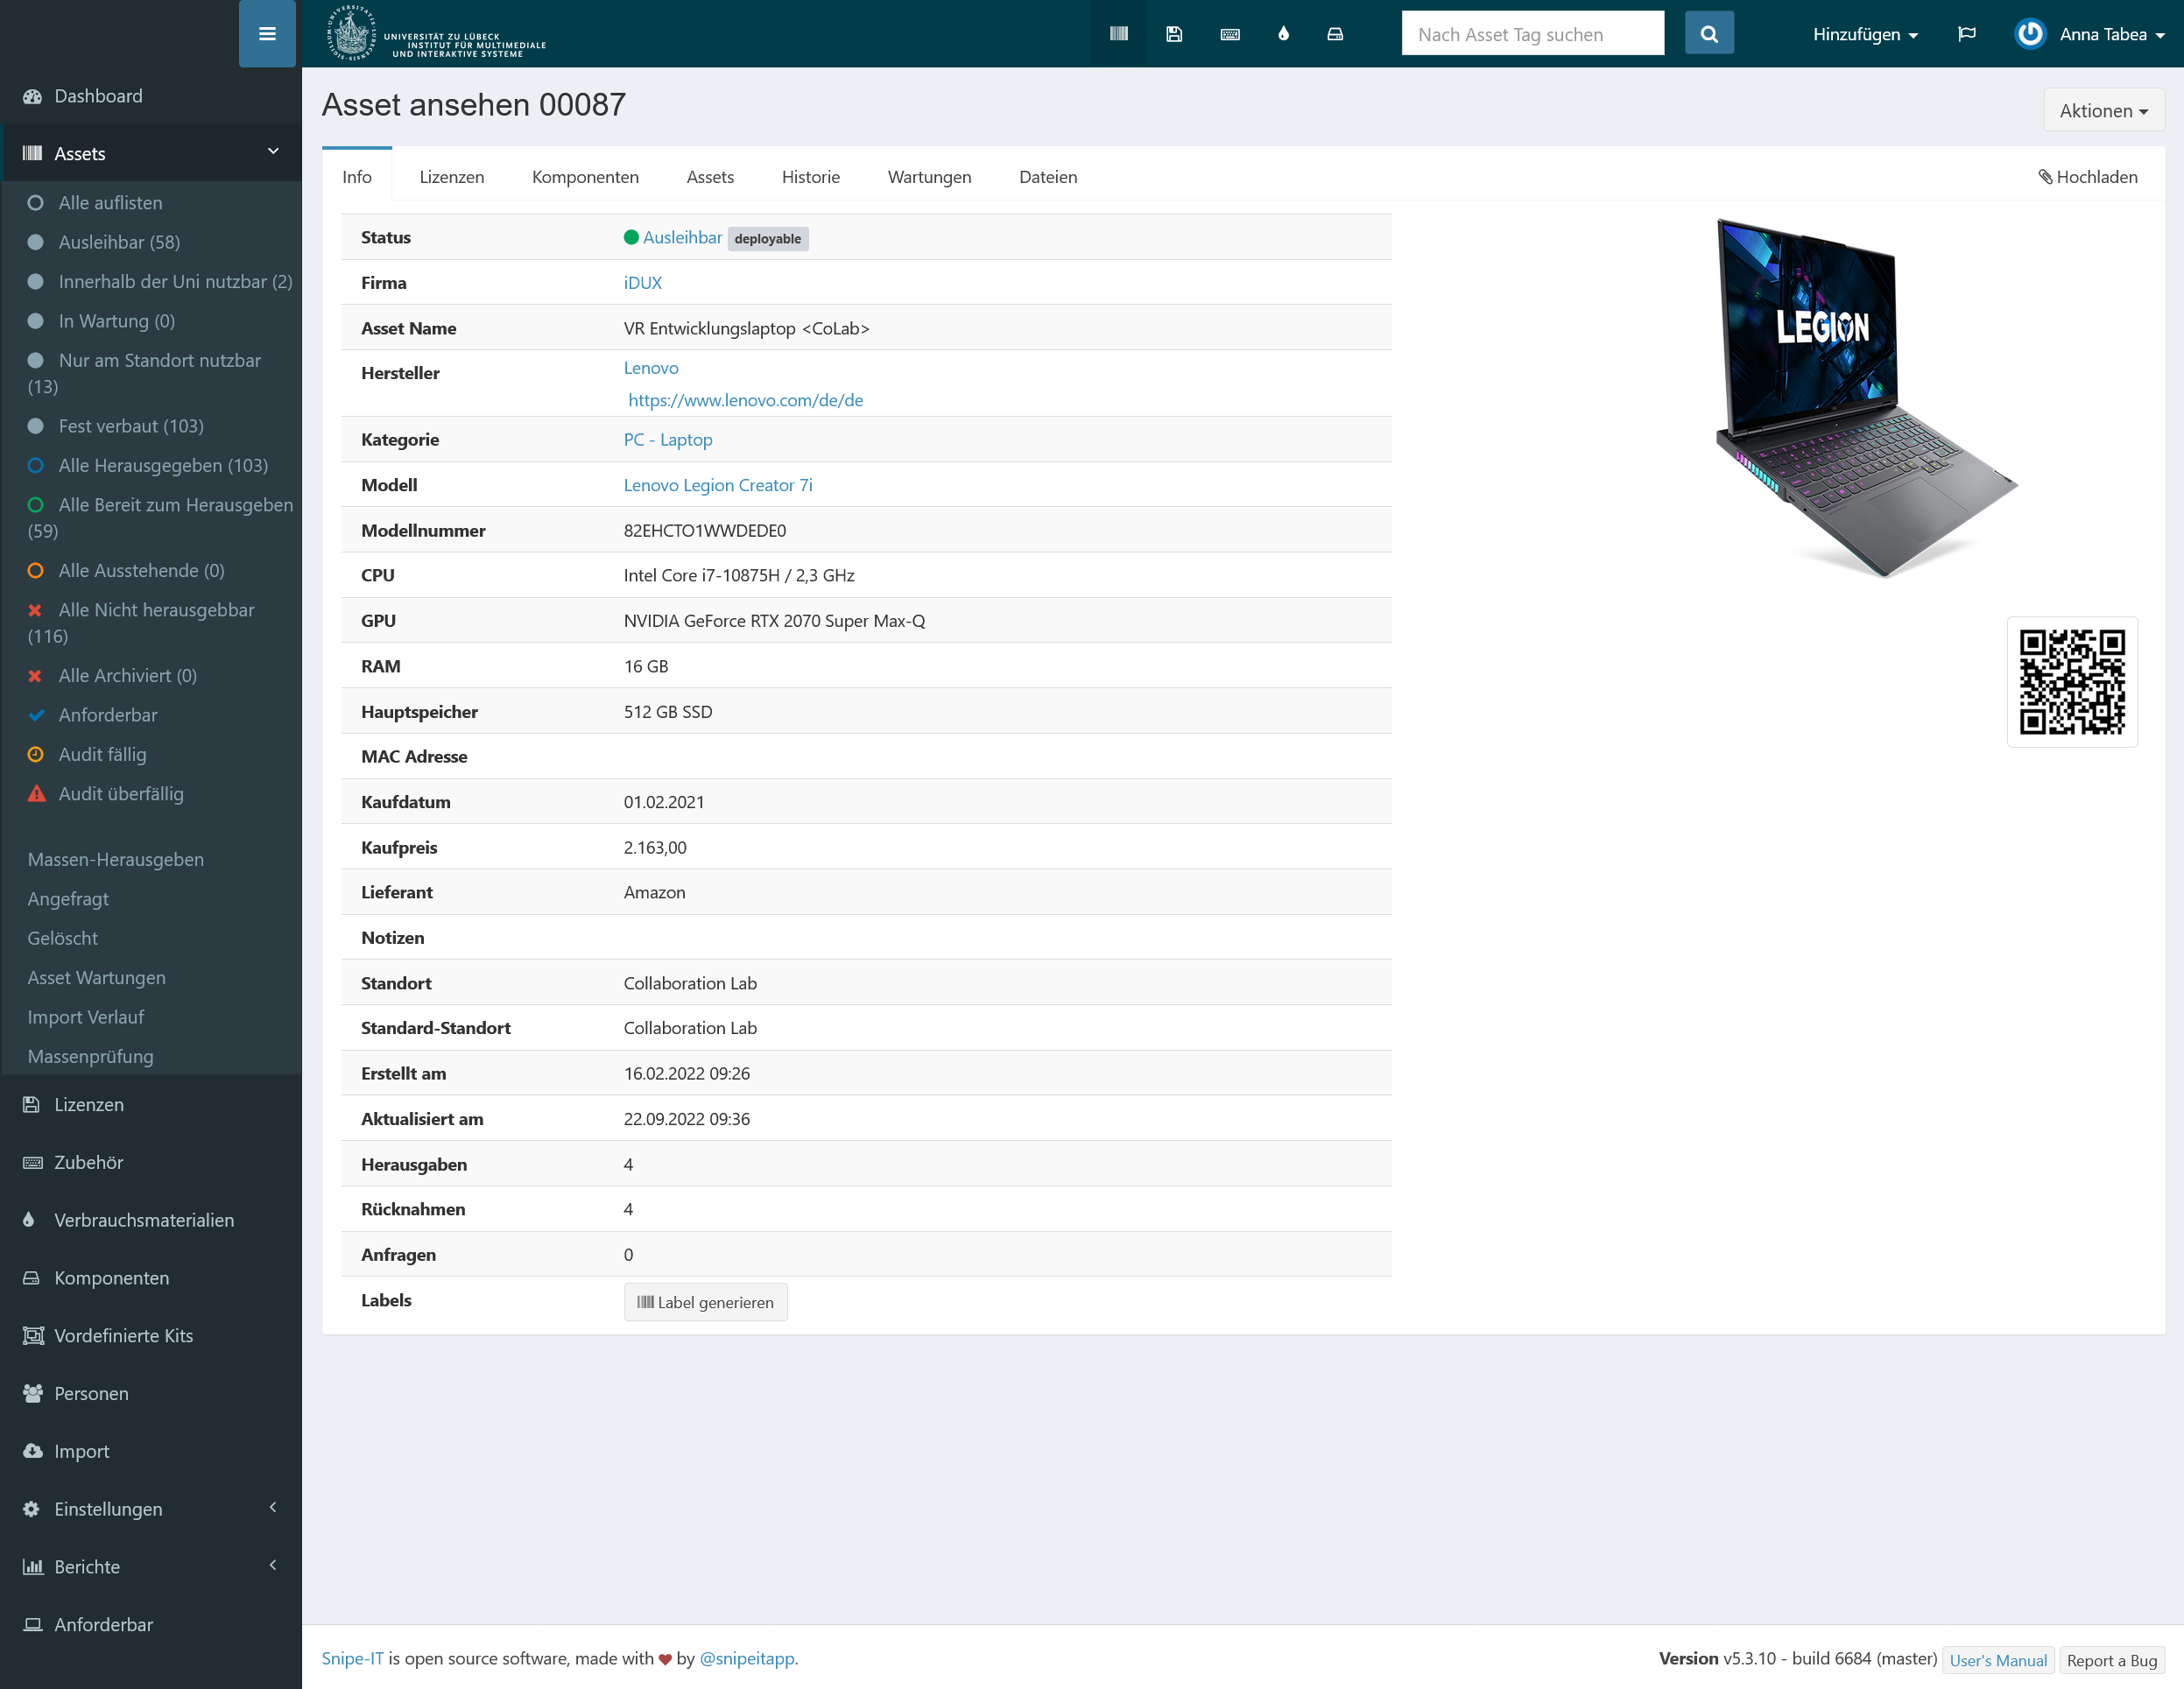
\includegraphics[scale=0.16]{Bilder/Screenshot 2022-10-14 at 11-26-25 Asset ansehen 00087 Ausleihmanagement.png}
    \label{fig:p4}
    \caption[Assetansicht in Snipe-IT]{Assetansicht in Snipe-IT}
\end{figure}

Milas Gruppe stellt am Dienstag fest, dass ihnen der Ausleihzeitraum nicht ausreicht und möchte
diesen daher um einen Tag verlängern. Dafür öffnet sie die Ausleih-App und sieht auf dem Dashboard
unter \textit{Laufende} ihre Reservierungen. Daraufhin ändert sie die Daten der beiden Materialien
auf Donnerstag um 9:00 Uhr. Am Donnerstag um 9:00 Uhr wartet Mila bereits auf Georg, welcher die
Materialien entgegennimmt und in seinem Büro die Rückgabe bestätigt.

\begin{figure}[h]
    \centering
    \includegraphics[scale=0.3]{Bilder/Prototyp/Übersicht.png}\hspace{2em}
    \includegraphics[scale=0.3]{Bilder/Prototyp/Übersicht1.png}
    \label{fig:p4}
    \caption[Mockup: Kategorien, Assets, Assetdetails]{Kategorien (l), Assetdetails (r)}
\end{figure}

Im vierten Semester möchte Mila das Mikrofon für das Modul: \textit{\ac{ide}} ausleihen, um wieder
ein Voiceover aufnehmen zu können. Sie findet das Mikrofon unter \textit{zurückgegeben} und
leiht das Material erneut aus.

\begin{figure}[h]
    \centering
    \includegraphics[scale=0.3]{Bilder/Prototyp/Übersicht.png}\hspace{2em}
    \includegraphics[scale=0.3]{Bilder/Prototyp/Übersicht1.png}
    \label{fig:p4}
    \caption[Mockup: Kategorien, Assets, Assetdetails]{Kategorien (l), Assetdetails (r)}
\end{figure}